\chapter{Elektrostatik}

\section{Grundgleichungen und elektrostatisches Potential}

In der Elektrostatik betrachten wir, wie der Name schon andeutet, zeitunabhängige Felder. Dementsprechend kann man als erste Konsequenz daraus folgern, dass $\dot{\vec{E}} = 0$ und $\dot{\vec{B}} = 0$ ist. Fallen nun in den \textsc{Maxwell}-Gleichungen alle Beiträge mit $\dot{\vec{E}}$ und $\dot{\vec{B}}$ weg, kann man die Felder $\vec{E}$ und $\vec{B}$ getrennt voneinander betrachten. Laienhaft gesprochen entkoppeln wir die Phänomene \grqq Elektrizität\grqq und "Magnetismus". Des Weiteren betrachten wir in der Elektrostatik nur ruhende Ladungen, woraus folgt, dass außerdem $\vec{j}=0 \Rightarrow \vec{B}=0$ ist.\

Damit erhalten wir aus der dritten \textsc{Maxwell}-Gleichung, dass rot $\vec{E} = 0$ gilt, wodurch das Einführen eines Potentials für $\vec{E}$ möglich wird:

\begin{equation*}
\vec{E} =: \ -\grad \varphi
\end{equation*}

Mit div $\vec{E} = \frac{\rho}{\epsilon_0}$ erhält man daraus die \textbf{\textsc{Poisson}-Gleichung} der Elektrostatik:

\begin{empheq}[box=\highlightbox]{equation*}
\laplace\varphi = - \frac{\rho\vphantom{\big|}}{\epsilon_0\vphantom{\big|}}
\end{empheq}

Für $\laplace\varphi = 0$ nennt man die \textsc{Poisson}-Gleichung auch \textbf{\textsc{Laplace}-Gleichung}.

\section{Kugelsymmetrische Ladungsverteilung}

Für eine kugelsymmetrische Ladungsverteilung gilt:

\begin{equation*}
\rho(\vec{r}) = \rho(|\vec{r}|) = \rho(r) \; \Rightarrow \; \varphi(\vec{r}) = \varphi(r)
\end{equation*}

Dem kann man entnehmen, dass die Äquipotentialflächen Kugelflächen sein müssen und somit der Gradient von $\varphi$ auch parallel zum Ortsvektor stehen muss.($\vec{E}(\vec{r}) = \vec{E}(r)\vec{e}_r$)\\
Für das $\vec{E}$-Feld gilt weiterhin:

\begin{equation*}
\epsilon_0\oiint\limits_{\partial \text{Kugel}}\mathrm{d}\vec{A}\cdot\vec{E} \; \overset{\vec{A}\parallel\vec{E}}{=} \; \epsilon_0\oiint\limits_{\partial \text{Kugel}}\mathrm{d} A \cdot E = 4\pi\epsilon_0\cdot r^2 \cdot E(r) = Q_{\mathrm{in}}(r)
\end{equation*}

Damit ergibt sich für das $\vec{E}$-Feld und das Potential:

\begin{empheq}[box=\highlightbox]{align*}
\vec{E}(r) &= \frac{Q_{\mathrm{in}}(r)}{4\pi\epsilon_0\cdot r^2} \cdot \vec{e}_r\\
\ \\
\varphi(r) &= \frac{Q_{\mathrm{in}}(r)}{4\pi\epsilon_0\cdot r} + \varphi_0 \quad \text{ mit } \quad \varphi_0 = \varphi(r \rightarrow 0)
\end{empheq}

\section[Feld einer beliebigen Ladungsverteilung]{Feld einer beliebigen räumlich begrenzten Ladungsverteilung}

\begin{enumerate}
\item \textbf{Punktladung bei} $\vec{r}_0$:
\begin{equation*}
\varphi(\vec{r}) = \frac{Q}{4\pi\epsilon_0 \ |\vec{r}-\vec{r}_0|}
\end{equation*}


\item \textbf{Mehrere Punktladungen} (Superpositionsprinzip anwendbar wegen Linearität der \textsc{Maxwell}-Gleichungen):
\begin{equation*}
\varphi(\vec{r}) = \sum\limits_i \ \frac{Q_i}{4\pi\epsilon_0 \ |\vec{r}-\vec{r}_i|}
\end{equation*}

\item \textbf{Kontinuierliche Ladungsverteilung}:
\begin{empheq}[box=\highlightbox]{equation*}
\varphi(\vec{r}) = \Int{\vphantom{a}}{\vphantom{a}}{V'} \ \frac{\rho(\vec{r}')}{4\pi\epsilon_0 \ |\vec{r}-\vec{r}'|}
\end{empheq}
\end{enumerate}

Die allgemeine Gleichung für die kontinuierliche Ladungsverteilung ergibt sich aus der Lösung der \textsc{Poisson}-Gleichung mithilfe der bekannten \textsc{Green}'schen Funktion für eine Punktladung der Größe 1:\quad $G(\vec{r}) = \frac{1}{4\pi\epsilon_0 \cdot |\vec{r}|}$\

\begin{align*}
-\epsilon_0 \cdot \laplace\varphi &= \rho\\
\Rightarrow -\epsilon_0 \cdot \laplace G(\vec{r}) &= \delta(\vec{r})\\
\end{align*}

Dabei gilt: $G(\vec{r},\vec{r}') = G(\vec{r}-\vec{r}')$ aufgrund der Translationsinvarianz der \textsc{Green}-Funktion.

\begin{equation*}
\Rightarrow \varphi(\vec{r}) = \int\mathrm{d}V' \ G(\vec{r}-\vec{r}')\cdot\rho(\vec{r}') = \frac{1}{4\pi\epsilon_0} \ \int\mathrm{d}V' \ \frac{\rho(\vec{r}')}{|\vec{r}-\vec{r}'|}
\end{equation*}
\ \\

Aus dieser allgemeinen Form lässt sich natürlich auch im umgekehrten Falle das $\vec{E}$-Feld einer Punktladung in $\vec{r}_0$ herleiten. Dafür muss nur $\rho(\vec{r}) = Q\cdot\delta(\vec{r}-\vec{r}_0)$ gesetzt werden:

\begin{equation*}
\varphi(\vec{r}) = \int\mathrm{d}V' \ \frac{\rho(\vec{r}')}{4\pi\epsilon_0 \cdot |\vec{r}-\vec{r}'|} = \ \frac{Q}{4\pi\epsilon_0} \ \underbrace{\int\mathrm{d}V' \ \frac{\delta(\vec{r}'-\vec{r}_0)}{|\vec{r}-\vec{r}'|}}_{=\frac{1}{|\vec{r}-\vec{r}_0|}}
\end{equation*}

\section{Feld eines elektrischen Dipols}

\begin{wrapfigure}[17]{r}[0cm]{0cm}
	\raisebox{0pt}[\dimexpr\height-1\baselineskip\relax]{
		\colorbox{hgrey}{
			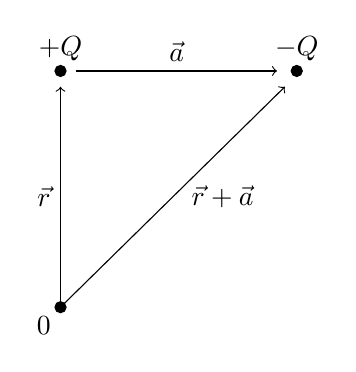
\begin{tikzpicture}
			
				 \draw[->](0,0)-- node[left]{$\vec{r}$} (0,2.8) ;
				 \draw[->](0,0)--node[right]{$\ \vec{r}+\vec{a}$}(2.85,2.8);
				 \draw[->](0.2,3)-- node[above]{$\vec{a}$}(2.75,3);
				 \filldraw[black] (0,0) circle (2pt) node[below left]{$0$};
				 \filldraw[black] (0,3) circle (2pt) node[above]{$+Q$};
				 \filldraw[black] (3,3) circle (2pt) node[above]{$-Q$};
			
			
			\end{tikzpicture}
		}
	}
	\caption{elektrischer Dipol}
\end{wrapfigure}
Ein Dipol besteht aus zwei gleich großen, entgegengesetzt geladenen Ladungen $\pm Q $, welche  einen festen Abstand $\vec{a}$ voneinander entfernt sind. Daher ergibt es Sinn, als charakteristische Eigenschaft des Dipols das \textbf{Dipolmoment} $\vec{p}$ wie folgt zu definieren:

\begin{empheq}[box=\highlightbox]{equation*}
\vec{p} := Q \cdot \vec{a}\vphantom{\Bigg|}
\end{empheq}

\begin{equation*}
\text{Dipollimit: } \quad |\vec{a}| \ \rightarrow \ 0, \ Q \ \rightarrow \ \infty 
\end{equation*}

\begin{equation*}
\Rightarrow \ |\vec{p}| = \ \text{const.}
\end{equation*}

Für das Potentialfeld eines solchen Dipols gilt offensichtlich:

\begin{equation*}
\varphi(\vec{r}) = \frac{Q}{4\pi\epsilon_0}\cdot\left(\frac{1}{|\vec{r}|} - \frac{1}{|\vec{r}+\vec{a}|}\right)
\end{equation*}

Für große Abstände von diesem Dipol, d.h. $\vec{r}\gg\vec{a}$ wollen wir das Potentialfeld \textsc{Taylor}-entwickeln, um besser mit ihm arbeiten zu können.\
Dazu betrachten wir den Term $\frac{1}{|\vec{r}+\vec{a}|}$ ein wenig genauer:\\

\begin{equation*}
\frac{1}{|\vec{r}+\vec{a}|} \cong \frac{1}{|\vec{r}|} + \left(\vec{a}\cdot\pdiff{}{\vec{r}}\right) \ \frac{1}{|\vec{r}|} = \frac{1}{|\vec{r}|}-\vec{a}\cdot\frac{\vec{r}}{|\vec{r}|^3}
\end{equation*}
\ \\
Damit gilt für das Potential:

\begin{empheq}[box=\highlightbox]{equation*}
\varphi(\vec{r})=\frac{Q\vphantom{\big|}}{4\pi\epsilon_0\vphantom{\big|}}\left(\frac{1}{r}-\frac{1}{r}-\left(\vec{a}\cdot\pdiff{}{\vec{r}}\right)\frac{1}{r}\right) = \frac{\vec{p}\cdot\vec{r}}{4\pi\epsilon_o\cdot r^3}
\end{empheq}

und das $\vec{E}$-Feld:

\begin{align*}
\vec{E}(\vec{r}) &= - \nabla \varphi = \frac{1}{4\pi\epsilon_0}\ \nabla \left(\vec{p}\cdot\nabla\right)\ \frac{1}{r} = \frac{\vec{p}}{4\pi\epsilon_0}\ \underbrace{\left(\nabla \circ \nabla\right)\ \frac{1}{r}}_{(*)}\\
\alignedbox{\hphantom{a}\vec{E}(\vec{r})}{= \frac{1}{4\pi\epsilon_0}\ \frac{3(\vec{p}\cdot\vec{r})\vec{r} - \vec{p}r^2}{r^5}\hphantom{a}}\\
\ \\
\text{mit}\quad (*) &= \left(\pdiff{}{\vec{r}} \circ \pdiff{}{\vec{r}}\right)\frac{1}{|\vec{r}|} = - \pdiff{}{\vec{r}}\circ\frac{\vec{r}}{|\vec{r}|^3} = \frac{3\vec{r}\circ\vec{r}-\mathbbm{1}\cdot\vec{r}^2}{|\vec{r}|^5}
\end{align*}
\ \\

\section[Fernfeld einer Ladungsverteilung]{Fernfeld einer räumlich eingegrenzten Ladungsverteilung}

\begin{wrapfigure}[]{l}[0cm]{0cm}
	\raisebox{0pt}[\dimexpr\height-1\baselineskip\relax]{
		\colorbox{hgrey}{
			\begin{tikzpicture}
			
			\filldraw[pattern=north west lines]  plot[smooth, tension=.8] coordinates {(0,1) (1,0) (3,1.5) (1.5,2) (0,1)};	
			\draw[|-|] (-1,0) -- node[left]{$a$} (-1,2);
			\draw  (2,-0.5)node[below]{$\rho(\vec{r'})$} -- (1.7,0.5);
			\draw[->] (2,1) -- (3,3) node[above]{$\vec{r}$};
			
			
			\end{tikzpicture}
		}
	}
	\caption{Verteilung}
\end{wrapfigure}

Wenn man das Fernfeld einer räumlich begrenzten Ladungsverteilung ermitteln möchte, spricht man in diesem Zusammenhang auch immer von der sogenannten \textbf{Multipolentwicklung}.

Wir betrachten nun eine räumlich eingegrenzte Ladunugsverteilung der Dichte $\rho$, für die zunächst einmal allgemein gilt:

\begin{equation*}
\varphi\left(\vec{r}\right) = \frac{1}{4\pi\epsilon_0}\cdot\int\d V \frac{\rho(\vec{r}')}{|\vec{r}-\vec{r}'|}
\end{equation*}

Unter der Annahme, dass $|\vec{r}| \gg \ a$ gilt (wobei $a$ die größte räumliche Ausdehnungsrichtung der Ladungsverteilung ist), werden wir nun den Term $\frac{1}{|\vec{r}-\vec{r}'|}$ entwickeln:
\newpage
\begin{equation*}
\frac{1}{|\vec{r}-\vec{r}'|} = \sum_{n=0}^{\infty} \; \frac{1}{n!}\left(-\vec{r}'\cdot\pdiff{}{\vec{r}}\right)^n \ \frac{1}{r} = \frac{1}{r} + \frac{\vec{r}'\cdot\vec{r}}{r^3} + \frac{1}{2} \ \frac{3 (\vec{r}'\cdot\vec{r})^2 - \vec{r}'^2 \ \vec{r}^2}{r^5} + \dotsc
\end{equation*}

\begin{align*}
\Rightarrow \quad \varphi(\vec{r}) &= \frac{1}{4\pi\epsilon_0} \left[ \frac{1}{r}\int\d V' \rho(\vec{r}') + \frac{\vec{r}}{r^3} \int\d V' \vec{r}' \rho(\vec{r}') + \sum_{i,j} \ \frac{x_i x_j}{r^5} \ \int\d V' \rho(\vec{r}') \ (3x_i'x_j' - \delta_{ij}\vec{r}'^2) + \dotsc\right] \\
\alignedbox{\hphantom{a}}{= \frac{1\vphantom{\big|}}{4\pi\epsilon_0\vphantom{\big|}} \left[\frac{Q}{r} \quad + \quad \frac{\vec{r}\cdot\vec{p}}{r^3} \quad + \quad \frac{1}{2}\frac{\vec{r}\cdot \tens{D} \cdot\vec{r}}{r^5} \quad + \quad \dotsc \quad \right]\hphantom{a}}\\
& \hspace{1.35cm} {\scriptstyle \sim\frac{1}{r}} \hspace{1.15cm} {\scriptstyle \sim \frac{1}{r^2}} \hspace{2cm} {\scriptstyle\sim\frac{1}{r^3}}
\end{align*}

Die einzelnen Summanden bezeichnet man auch als \textbf{Multipolmomente} einer Ladungsverteilung:

\begin{align*}
\mathrm{Monopol:}& \qquad Q = \int\d V \rho(\vec{r})\\
\mathrm{Dipol:}& \qquad \vec{p} = \int\d V \rho(\vec{r})\vec{r}\\
\mathrm{Quadrupol:}& \qquad \tens{D} = \int\d V \rho(\vec{r}) \ (3\vec{r}\circ\vec{r}-\mathbbm{1}\vec{r}^2)\\
\mathrm{Oktupol:}& \qquad \dotsc\\
\vdots \qquad &
\end{align*}

Im Allgemeinen hängen die Multipolmomente vom Bezugspunkt ab, nur das erste nicht verschwindende Moment ist unabhängig vom selbigen.\\
Der Quadrupol-Tensor $\tens{D}$ hat dabei folgende Eigenschaften:\\

\begin{itemize}
\item $\bm{D}_{ij} = \bm{D}_{ji}$, insbesondere gilt:

\begin{equation*}
\operatorname{Spur}\tens{D} = \sum_j \bm{D}_{jj} = \Int{}{}{V}(3\vec{r}^2 - 3 \vec{r}^2) =0
\end{equation*}

\item $\tens{D}$ hat 5 unabhängige Komponenten
\item $\tens{D}$ kann hauptachsentransformiert werden
\item aus $\operatorname{Spur} \tens{D}=0$ folgt $\tens{D}=0$ für Kugel und Kegel 
\end{itemize}
\ \\

Aufgrund der der charakteristischen Richtungsabhängigkeit ist es sinnvoll, das Potential der Ladungsverteilung mit Kugelflächenfunktionen zu entwickeln. Ausgangspunkt ist hierbei wieder das allgemeine Potential für eine beliebige Ladungsverteilung: 

\begin{equation*}
\varphi(\vec{r}) = \frac{1}{4\pi\epsilon_0}\int\d V' \frac{\rho(\vec{r})}{|\vec{r}-\vec{r}'|} = \int\d V' G(\vec{r}-\vec{r}')\rho(\vec{r}')
\end{equation*}

Wobei $G$ die \textsc{Green}'sche Funktion ist, welche die \textsc{Poisson}-Gleichung mit $\delta$-förmiger Inhomogenität löst:

\begin{equation*}
-\epsilon_0 \ \laplace G(\vec{r}) = \delta(\vec{r})
\end{equation*}

Als nächstes separieren wir die Winkel- und Richtungsabhängigkeit des Differentialoperators $\laplace$, welches sich am besten explizit in Kugelkoordinaten vornehmen lässt.

\begin{equation*}
\laplace = \frac{1}{r} \pddiff{}{r}  \; +\; \underbrace{\frac{1}{r^2 \sin\theta} \pdiff{}{\theta} \sin\theta \; \pdiff{}{\theta} \; + \; \frac{1}{r^2 \sin^2\theta} \ \pddiff{}{\phi}}_{=: \frac{1}{r^2}\Lambda(\theta,\phi)}
\end{equation*}

Nun wenden wir auf die Differentialgleichung

\begin{equation*}
\Lambda \ Y(\theta,\phi) \; = \; -l(l+1) \ Y(\theta,\phi) \qquad l \in \mathbb{N}
\end{equation*}

den Separationsansatz $Y(\theta,\phi) = P(\theta)\cdot Q(\phi)$ an und erhalten zunächst für $Q(\phi)$:

\begin{align*}
\ddiff{}{\phi}Q(\phi) &= - m^2 Q(\phi)\\
\Rightarrow Q &= e^{im\phi} \qquad \text{ mit } \quad m \in [-l,l] \subset \mathbb{Z}
\end{align*}

Substituieren wir nun oben $\cos\theta = x$, so führt dies auf eine verallgemeinerte \textbf{\textsc{Legendre}-Differentialgleichung} für $P(x)$

\begin{equation*}
\left(\diff{}{x} \ \left(1+x^2\right) \ \diff{}{x} \ \left(-\frac{m^2}{1-x^2} + l(l+1)\right)\right) \ P_l^m(x) = 0
\end{equation*}

Es genügt diese für $m=1$ zu lösen, denn:

\begin{equation*}
P_l^m(x) = (-1)^m(1-x)^{\frac{m}{2}} \ \left(\diff{}{x}\right)^{|m|} P_l(x)
\end{equation*}

Somit bleibt nur noch folgende \textsc{Legendre}-Differentialgleichung übrig:

\begin{equation*}
(1-x^2) P_l'' \ - \ 2x \ P_l' \ + \ l(l+1) \ P_l \ = \ 0
\end{equation*}

Deren Lösungen $P_l$ sind sogenannte \textbf{\textsc{Legendre}-Polynome}:

\begin{equation*}
P_l(x) = \frac{1}{2^l l!} \ \left(\diff{}{x}\right)^l \ (x^2+1)^l \qquad l\in \mathbb{N}
\end{equation*}

(Die ersten $P_l$ lauten explizit: $P_0(x) =1, \; P_1(x) = x, \; P_2(x) = \frac{1}{2}(3x-1), \dotsc$)
Nun erhalten wir aus $P$ und $Q$ unsere ursprüngliche, separierte Funktion $Y(\theta,\phi)$:

\begin{equation*}
Y_{lm}(\theta,\phi) = \sqrt{\frac{2l + 1}{4\pi} \ \frac{(l-|m|)!}{(l+|m|)!}} \ P_l(\cos\theta) \ e^{im\phi}
\end{equation*}

(Die ersten $Y_{lm}$ lauten explizit: $Y_{00} = \frac{1}{\sqrt{4\pi}}, \; Y_{10} = \sqrt{\frac{3}{4\pi}}\cos\theta, \; Y_{1,\pm1} = \mp \sqrt{\frac{3}{8\pi}}\sin\theta \ e^{i\phi}$\
\\
\ \\
\underline{Bemerkung zu den $Y_{lm}$:}\\
\ \\
Die $Y_{lm}$ sind sogenannte \textbf{Kugelflächenfunktionen} und Lösungen der Differentialgleichung

\begin{align*}
\left(\frac{1}{\sin\theta}\pdiff{}{\theta} \ + \ \sin\theta \pdiff{}{\theta} \ + \ \frac{1}{\sin^2\theta} \pddiff{}{\phi} \ + \ l(l+1)\right) \ Y_{lm}(\theta,\phi) = 0\\
l \in \mathbb{N}, m \in [-l,l]
\end{align*}

Anschaulich gesprochen sind die Kugelflächenfunktionen die Eigenfunktionen des Winkelanteils des \textsc{Laplace}-Operators und daher sehr gut als Darstellungsbasis für sämtliche Funktionen auf Kugeloberflächen geeignet. Man kann auch zeigen, dass sie nicht nur eine beliebige Basis, sondern sogar eine Orthonormalbasis sind; dazu überprüfen wir zunächst die Orthogonalität der Basiselemente zueinander:

\begin{equation*}
\langle Y_{lm},Y_{l'm'}\rangle =: \int_{-1}^1\d(\cos\theta)\int_{0}^{2\pi}\d\phi \ Y^{*}_{lm}(\theta\phi) Y_{lm}(\theta\phi) = \delta_{ll'}\delta_{mm'}
\end{equation*}

Nach bekannter Vorgehensweise lässt sich nun jede beliebige Funktion $f$ auf einer Kugeloberfläche aus den $Y_{lm}$ darstellen:

\begin{align*}
f(\theta,\phi) &= \sum_{l=0}^{\infty} \sum_{m=-l}^{l} f_{lm} Y_{lm}(\theta,\phi)\\
\text{mit } f_{lm} &= \langle Y_{lm},f\rangle = \int\d(\cos\theta) \int\d\phi \ Y^{*}_{lm}(\theta,\phi)f(\theta,\phi)
\end{align*}

Somit lässt sich auch mit ihnen die allgemeine Lösung der \textsc{Laplace}-Gleichung $\laplace\varphi=0$ darstellen: 

\begin{equation*}
\varphi(r,\theta,\phi) = \sum_{l=0}^{\infty}\sum_{m=-l}^{l} \left(A_l \cdot r^l + B_l \cdot r^{-l-1}\right) Y_{lm}(\theta,\phi)
\end{equation*}

Wir können nun zur Entwicklung von $\frac{1}{|\vec{r} - \vec{r}'|}$ zurückkehren:

\begin{align*}
\frac{1}{|\vec{r} - \vec{r}'|} = \sum_{l=0} \left(A_l \cdot r^l + B_l \cdot r^{-l-1}\right) P_l(\cos\gamma) \quad \text{ mit } \gamma = \sphericalangle\left(\vec{r},\vec{r}'\right)\\
(\gamma\text{ ohne $\phi$-Abhängigkeit wegen axialer Symmetrie)}
\end{align*}

Wähle nun für die $A_l, B_l$, dass $\vec{r}\parallel\vec{r}'$ ist und führe so die Entwicklung fort

\begin{align*}
\frac{1}{|\vec{r}-\vec{r}'|} &= \sum_{l=0}^{\infty} \ \frac{1}{l!} \left(\-r_{<}\diff{}{r_{<}}\right)^l \ \frac{1}{r_{>}} \qquad \text{ mit } r_{<} := \min\{r,r'\}, \ r_{>} \text{ analog}\\
&= \frac{1}{r_{<}}\sum_{l=0}^{\infty} \ \left(\frac{r_{>}}{r_{<}}\right)^l\\
&=  \sum_{l=0}^{\infty} \frac{r_{>}}{r_{<}^{l+1}} \ P_l (\cos\gamma)\\
\\
P_l (\cos\gamma) &= \frac{4\pi}{2l+1}\sum_{m=-l}^{l}  Y^{*}_{lm}(\theta',\phi')Y_{lm}(\theta,\phi)\\
& \quad\left(\cos\gamma = \cos\theta\cos\theta' \ + \ \sin\theta\sin\theta'\cos(\phi-\phi')\right)\\
\\
\Rightarrow \frac{1}{|\vec{r}-\vec{r}'|} &= 4\pi \sum_{l=0}^{\infty}\sum_{m=-l}^{l} \frac{1}{2l+1}\ \frac{r_{>}^l}{r_{<}^{l+1}} Y^{*}_{lm}(\theta',\phi')Y_{lm}(\theta,\phi)
\end{align*}

Wir haben nun $\frac{1}{|\vec{r}-\vec{r}'|}$ vollständig faktorisiert und können nun das Potential einer Ladungsverteilung aufstellen:\\

\begin{empheq}[box=\highlightbox]{equation*}
\varphi (\vec{r}) = \frac{1}{4\pi\epsilon_0} \sum_{l,m} \ \sqrt{\frac{4\pi}{2l +1}} \ \frac{Y_{lm}(\theta,\phi)}{r^{l+1}} \ \underbrace{\Int{}{\vphantom{\Big|}}{V'} \  \rho(\vec{r}) \  Y_{lm}^{*}(\theta',\phi') \ {r'}^l \sqrt{\frac{4\pi}{2l+1}}}_{q_{lm} \hat{=} \text{ Multipolmomente}}
\end{empheq}
\newpage
Aus dem allgemeinen Ausdruck $q_{lm}$ für die Multipolmomente können wir nun auch die uns bereits bekannten Momente ableiten:

\begin{align*}
q_{00} &= \sqrt{4\pi}\int\d V' \ \rho(\vec{r}') \ Y_{00} = Q
\\
q_{10} &= \int\d V' \ \rho(\vec{r}') \ \underbrace{r'\cos\theta'}_{z'} = p_z\\
q_{1,\pm 1} &= \pm \frac{1}{\sqrt{2}} \ \int\d V' \ \rho(\vec{r}')  \ r'\sin\theta' \; e^{i\phi'} = (p_x \mp i p_y) \cdot \frac{1}{\sqrt{2}}\\
\\q_{2m} &\rightarrow \text{ 5 skalare Komponenten } \rightarrow \text{ Quadrupol}
\end{align*}

\section{Randbedingungen}

Die allgemeine Lösung der \textsc{Poisson}-Gleichung $\epsilon_0 \bigtriangleup \varphi = \rho$ hängt von ihren Randbedingungen ab. Die vollständige Lösung erhält man durch Addition der allgemeinen Lösung der zugehörigen homogenen Differentialgleichung und einer partikulären Lösung der inhomogenen Gleichung: $\quad \varphi = \varphi_p + \varphi_h$.\\
Es bietet sich an die Randbedingungen in den homogenen Teil einzubauen (bisher haben wir immer angenommen, dass $\varphi (\infty) = 0$). Mathematisch liefert uns eine einzige Randbedingung auf einem geschlossenen Rand R eine physikalisch eindeutige Lösung für eine Differentialgleichung 2. Ordnung, da es sich durch den geschlossenen Rand effektiv um zwei Randbedingungen handelt. Wir unterscheiden dabei verschiedene gängige Varianten sich dem Problem zu nähern:


\begin{enumerate}
\item $\varphi(R)$ ist gegeben\
\\
Diese Variante nennt man auch die \textsc{Dirichlet}-Randbedingung\

\item $\pdiff{\varphi}{n}(R)$ ist gegeben\
\\
\ \\
Diese Variante nennt man auch die \textsc{von-Neumann}-Randbedingung\
\\
\ \\
($\pdiff{\varphi}{n} := \pdiff{\varphi}{\vec{r}}\cdot\vec{e}_n = - \vec{E}_n$ ist dabei die Normalenableitung)\

\item $\alpha \varphi \ + \ \beta\pdiff{\varphi}{n}$ ist gegeben
\end{enumerate}

\section{Leiter im elektrischen Feld}

Bis jetzt hatten wir in der Elektrostatik nur ruhende Ladungen betrachtet. In Leitern  gibt es allerdings bewegliche Ladungen im Inneren. Diese befinden sich im Gleichgewicht bei $\vec{F}=0 \ \Rightarrow \vec{E}= 0$
Daraus kann man dieser folgern, dass $\varphi =$ \textit{const.} \ im Inneren des Leiters und auf der Leiteroberfläche gilt. Dafür muss gelten, dass $\rho = 0$ im Leiterinneren ist. Außerdem folgt direkt, dass $\vec{E} = -\pdiff{\varphi}{\vec{r}}$ senkrecht zur Oberfläche stehen muss und das es ausschließlich von \textbf{Oberflächenladungen} erzeugt wird. Um diese zu definieren betrachten wir ein Volumen $\Delta V$ auf dem Leiteroberflächenstück $\Delta \vec{A}$, welches die Ladung $\Delta Q$ in sich trägt.

\begin{equation*}
\epsilon_0 \oiint_{\partial\Delta V}\d\vec{A}\cdot\vec{E} = \Delta Q \quad \Rightarrow \quad \epsilon_0 \ \Delta\vec{A}\cdot\vec{E}_n = \Delta Q
\end{equation*}

Darüber können wir uns die \textbf{Flächenladungsdichte} $\sigma$ definieren, um die Oberflächenladungen beschreiben zu können:

\begin{align*}
\alignedbox{\hphantom{a}\sigma} {:= \frac{\Delta Q}{\Delta A} = \epsilon_0 \ E_n\vphantom{\Bigg|}\hphantom{a}}\\
Q  &= \iint\d A \cdot \sigma
\end{align*}

Die Oberflächenladungen werden durch äußere elektrische Felder bestimmt und schirmen das Leiterinnere von diesen Feldern ab.\
\\
\ \\
Betrachten wir nun den Innenraum eines Hohlleiters. Hier gilt genau wie bei einem normalen Leiter, dass auf der Leiteroberfläche das Potential konstant ist. Zudem ist der Innenraum ladungsfrei, woraus folgt, dass auch dort $\varphi$ =\textit{const.} \ gilt uns somit auch $\vec{E} = 0$. Dieses Prinzip ist auch als \textbf{\textsc{Faraday}'scher Käfig} bekannt.\
\\
Die Begründung für dieses Prizip kann man auch direkt aus den \textsc{Maxwell}-Gleichungen herleiten, denn es gilt div $\vec{E} = 0$ und rot $\vec{E} = 0$ im Inneren des Hohlleiters. Jede Feldlinie im Inneren müsste demzufolge auf dem Rand anfangen und enden. Für eine Integration entlang einer Feldlinie $\int\d \vec{r} \cdot \vec{E} = \Delta \varphi$ würde dies jedoch ein endliches $\Delta \varphi$ zwischen Anfangs- und Endpunkt liefern, welches im Widerspruch zu $\varphi$ = const. auf dem Rand stehen würde. Also muss $\vec{E} = 0$ im Inneren des Hohlleiters gelten.

\newpage
\underline{\textbf{Beispiele}}
\begin{enumerate}
\item \textbf{ Punktladung und ebene Leiterfläche}\\
\ \\
Wir betrachten eine Punktladung $Q$, welche sich im Abstand $a$ von einer ebenen Leiteroberfläche befindet. Letztere sei entlang der y-Achse unseres Koordinatensystems ausgerichtet, während sich $Q$ auf der x-Achse befindet.
Demzufolge erhalten wir die \textsc{Poisson}-Gleichung:

\begin{equation*}
-\epsilon_0 \ \laplace\varphi = Q \ \delta(\vec{r}-a\vec{e}_x)
\end{equation*}

mit der Randbedingung $\varphi(x=0) = 0$ auf der Leiteroberfläche.\
Wir wissen, dass die Feldlinien der Punktladung senkrecht auf die Leiteroberfläche aufkommen müssen. Daher können wir uns fragen, wie man eben jenes Feldlinienbild beschreiben könnte. Man erhält es durch das Einbringen einer zweiten, gedachten Ladung $-Q$ bei $-a\vec{e}_x$, sodass die gesamte Anordnung für x$>0$ das gesuchte Feldlinienbild ergibt. Die imaginäre Punktladung bei $-a\vec{e}_x$ nennt man \textbf{Spiegelladung}. Die Begründung für dieses Phänomen ist, das das Einbringen einer Leiteroberfläche in ein gegebenes Potential $\varphi (\vec{r})$ entlang einer Äquipotentialfläche das Feld außerhalb des Leiters nicht ändert. Dort gilt weiterhin $-\epsilon_0 \laplace\varphi = \rho$ unverändert und die Randbedingungen sind effektiv identisch zu der Gleichung, welche das Feldlinienbild mithilfe der Spiegelladung beschreibt. Diese lautet hier:

\begin{equation*}
- \laplace\varphi = Q \left(\delta(\vec{r}-a\vec{e}_x) \ - \ \delta(\vec{r}+a\vec{e}_x)\right)
\end{equation*}

welche für das Potential liefert:

\begin{equation*}
\varphi = \frac{Q}{4\pi\epsilon_0} \left(\frac{1}{|\vec{r}-a\vec{e}_x|} \ - \ \frac{1}{|\vec{r}+a\vec{e}_x|}\right)
\end{equation*}
\newpage

\item \textbf{ Kugeloberfläche in einem asymptotisch homogenen Feld}\\
\ \\
Wir betrachten eine leitende Kugel mit dem Radius $R$, welche sich im Ursprung des Koordinatensystems in einem homogenen elektrischen Feld $\vec{E}_0$ befindet. Für $|\vec{r}|>R$ gilt dementsprechend: $\bigtriangleup\varphi = 0$ mit den Randbedingungen $\varphi(|\vec{r}| = R) = \varphi_0 := 0$ und $\varphi(|\vec{r}|\rightarrow\infty) = -\vec{E}_0\cdot\vec{r}$ (Homogenität des Feldes). Aus Symmetrieüberlegungen erhalten wir außerdem, dass $\varphi(\vec{r},R,\vec{E}_0)$ linear in $\vec{E}_0$ sein muss.\
Dementsprechend wählen wir den Ansatz $\varphi = -\vec{E}_0 \cdot\vec{r} \ G(r,R)$ mit den resultierenden Randbedingungen $G(r=R)=0$ und $G(r\rightarrow\infty
) =1$, welcher nach Einsetzen in die \textsc{Laplace}-Gleichung folgende homogene DGL für $G$ liefert:

\begin{equation*}
\laplace\varphi = -\vec{E}_0\cdot\vec{r} \ \left(\frac{4}{r} \ \diff{G}{r} \ + \ \ddiff{G}{r}\right) = 0
\end{equation*}
\ \\
Diese lösen wir mit dem Ansatz $G \sim r^n$:
\begin{align*}
& 4n + n(n+1) = 0\\
\Rightarrow & n_1 = 0, n_2=3\\
\Rightarrow & G = C_1 + \frac{C_2}{r^3}\\
\ \\
\text{Rb.: } & G(r\rightarrow\infty) = 1 \quad \Rightarrow \quad C_1 = 1\\
& G(r=R) = 0 \quad \Rightarrow \quad C_2 = -R^3 
\end{align*}

Also ergibt sich für $\varphi$:

\begin{equation*}
\varphi = \vec{E}_0\cdot\vec{r} \ + \ \frac{\vec{p} \cdot\vec{r}}{4\pi\epsilon_0 r^3} \quad
\text{ mit } \quad \frac{\vec{p}}{4\pi\epsilon_0} = \vec{E}_0 \cdot R^3
\end{equation*}

Das äußere elektrische Feld induziert also offensichtlich ein Dipolmoment in der Kugel, welches für den zusätzlichen Term in $\varphi$ verantwortlich ist.
\end{enumerate}
\newpage

\section{Mehrere Leiter}

Wir betrachten mehrere Leiter im Raum mit den Oberflächen $\mathcal{S}_i$. Erneut gilt die Tatsache, dass es keine Raumladungen gibt ($\bigtriangleup\varphi = 0$) und die Randbedingungen für die Leiteroberflächen $\varphi_i = \varphi$ auf den $\mathcal{S}_i. \ (\varphi_0 = 0$ wird willkürlich festgelegt)\\
Nun gilt aufgrund der Linearität der \textsc{Maxwell}-Gleichungen für das Gesamtpotential:

\begin{equation*}
\varphi (\vec{r}) = \sum_k \ G_k(\vec{r}) \ \varphi_k
\end{equation*}

Die $G_k$ hängen dabei von der Geometrie der Leiteranordnung ab.\
Wenn wir nun die Quellen auf den $\mathcal{S}_i$ mit in die Betrachtung mit einbeziehen, erhalten wir: 

\begin{align*}
\sigma &= \epsilon_0 \vec{E}_n\big|_{\mathcal{S}_i}  = -\epsilon_0 \pdiff{\varphi}{n}\Bigg|_{\mathcal{S}_i} = - \epsilon_0 \sum_k \pdiff{G_K(\vec{r})}{n}\Bigg|_{\mathcal{S}_i} \ \varphi_k \\
\ \\
\Rightarrow Q_i &= \Oiint{\mathcal{S}_i}{}{A} \ \sigma = -\epsilon_0\sum_k\Oiint{\mathcal{S}_i}{}{\vec{A}}\  \cdot \ \pdiff{G_K(\vec{r})}{\vec{r}} \ \varphi_k\\
\alignedbox{\hphantom{a}Q_i}{=: \sum_k C_{ik} \varphi_k \quad \text{ mit } \quad C_{ik} = -\epsilon_0 \Oiint{\mathcal{S}_i}{\vphantom{A}}{\vec{A}} \ \cdot \ \pdiff{G_k}{\vec{r}}\hphantom{a}}
\end{align*}


Die $C_{ik}$ nennen wir die \textbf{Kapazitätskoeffizienten}. Für sie gilt $C_{ik} = C_{ki}$. Speziell für zwei sich umschließende Leiter ($\hat{=}$ Kondensator) folgt daraus:

\begin{equation*}
Q_1 = C_{11}\varphi_1 \quad (\text{und } Q_0 = -Q_1) \quad \hat{=} \quad \ Q=C \cdot U
\end{equation*}